\documentclass[12pt]{article}
\usepackage{geometry}                % See geometry.pdf to learn the layout options. There are lots.
\geometry{letterpaper}                   % ... or a4paper or a5paper or ... 
%\geometry{landscape}                % Activate for for rotated page geometry
\usepackage[parfill]{parskip}    % Activate to begin paragraphs with an empty line rather than an indent
\usepackage{daves,fancyhdr,natbib,graphicx,dcolumn,amsmath,lastpage,url}
\usepackage{amsmath,amssymb,epstopdf,longtable}
\usepackage{paralist}  % need to properly formulate standard answer blocks
\usepackage[final]{pdfpages}
\DeclareGraphicsRule{.tif}{png}{.png}{`convert #1 `dirname #1`/`basename #1 .tif`.png}
\pagestyle{fancy}
\lhead{CE 3305 Fluid Mechanics; Exercise Set 4}
\rhead{Name:\_\_\_\_\_\_\_\_\_\_\_\_\_\_\_\_\_\_\_\_\_\_\_\_\_\_\_\_\_\_\_\_\_\_}
\lfoot{REVISION A}
\cfoot{}
\rfoot{Page \thepage\ of \pageref{LastPage}}
\renewcommand\headrulewidth{0pt}
%%%%%%%%%%%%%%%%%%%%%%%%%%%%%%%%%%%%
\begin{document}
%%%%%%%%%%%%%%%%%%%%%%%%%%%%%%%%%%%
\begingroup
\begin{center}
{\textbf{{ CE 3305 Engineering Fluid Mechanics} \\ Exercise Set 4 \\ Summer 2015 -- GERMANY} }
\end{center}
\endgroup
\begingroup
~\newline

\begin{enumerate}
\item (Problem 3.7 pg 95)
Figure \ref{fig:MouseElephant} is a schematic of a hydraulic machine lifting an elephant using the weight of a mouse.
\begin{enumerate}[a)]
\item Derive an algebraic equation that gives the mechanical advantage of the hydraulic machine shown.  
Neglect piston friction and piston mass.
\item A mouse can have a mass of 25 grams while an elephant can have a mass of 7500 kilograms.   Determine the values of $D_1$ and $D_2$ so that a mouse can support an elephant.
\end{enumerate}
\begin{figure}[htbp] %  figure placement: here, top, bottom, or page
   \centering
   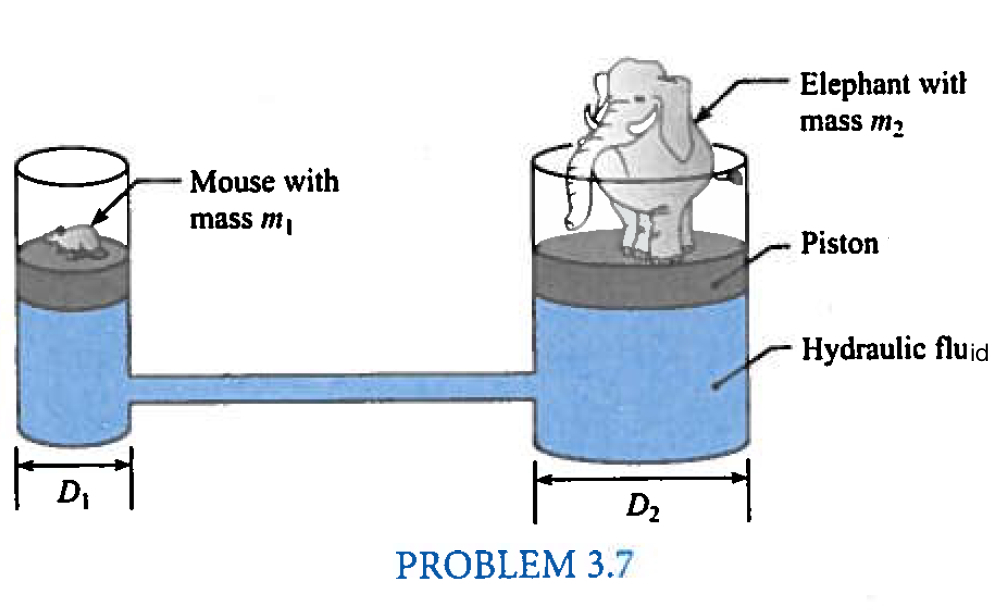
\includegraphics[width=5in]{MouseElephant.jpg} 
   \caption{Mechanical advantage using a hydraulic jack -- or a mouse supports a heffalump!}
   \label{fig:MouseElephant}
\end{figure}
\clearpage
~
\clearpage
\item (Problem 3.10 pg 95)
Imagine two tanks (both open to air).  Tank $A$ is filled to a depth $h$ with water.
Tank $B$ is filled to a depth $h$ with oil.
\begin{enumerate}[a)]
\item Which tank has the largest pressure?
\item Why?
\item Where in the tank does the largest pressure occur?
\end{enumerate}
\end{enumerate}


\end{document}  